\documentclass[11pt,fleqn]{article}

\setlength {\topmargin} {-.15in}
\setlength {\textheight} {8.6in}

\usepackage{amsmath}
\usepackage{amssymb}
\usepackage{color}
\usepackage{tikz}
\usetikzlibrary{automata,positioning,arrows}
\usepackage{diagbox}
\usepackage{stackrel}
\begin{document}


\textbf{Exercise 2.2.21:} Triplicates. Given three lists of N names each, devise a linearithmic algorithm
to determine if there is any name common to all three lists, and if so, return the first
such name.\\

\textbf{Solution:}
First, sort the array in ascending order so that it is easier to identify values/elements without repetition.\\

Then compare the values/elements of each array while increasing the index to be compared at, until finds a match. Kind of similar to the concept of how you try to merge arrays together in mergesort going little by little, incrementing each array index.

\begin{center}
	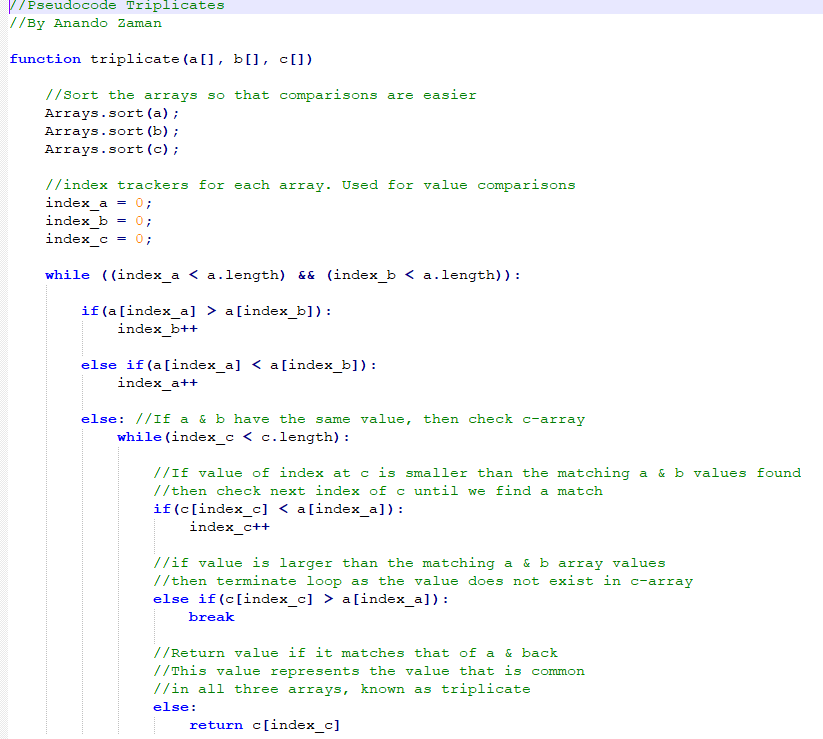
\includegraphics[scale = 0.8]{2.2.21.png}
	\end{center}

\end{document}
